\documentclass[12pt]{article}
\usepackage[utf8]{inputenc}
\usepackage{graphicx}
\usepackage{listings}
\usepackage{wrapfig}
\usepackage{subfigure}
\usepackage{hyperref}
\usepackage{amsmath}
\usepackage{indentfirst}
\usepackage[margin=1in]{geometry}

\title{\vspace{-8ex}Proposal:\\Browser-Based 3D Turtle}
\author{Nathan Walters\\nwalter2}
\date{\today}

\begin{document}

\maketitle

\section{Abstract}

My project will consist of a brower-based 3D turtle graphics application implemented with JavaScript and HTML5. It should work similarly to a standard 2D turtle system, with the logical extension that the turtle will be able to move along a third dimension. It will also allow the user to rotate and move the ``camera'' so as to be able to view the turtle's drawings from different perspectives.

\section{Background}

Turtle graphics refers to a relative cursor (or pen, if you will) that moves over a surface, leaving marks as it goes. At any given point in time, the turtle has a certain location and orientation on its drawing plane. The turtle can be given commands to move relative to its current position; for instance, one could tell the turtle to ``turn right 90 degrees'' or ``move forward 15 units''. In this way, turtle graphics is primarily vector-based. This is different from an absolute graphics system, where geometric figures would be described by absolute coordinates. However, because a digital turtle is still moving within an absolute coordinate space, some turtle graphics implementations include commands such as ``move to the location (10,5)'' which can make it easier to implement certain things.

The turtle was originally a physical robot that could drive around, making marks on paper with a retractable pen as it went. Seymour Papert popularized the idea of turtle graphics in the 1980s when he added support for turtle graphics to the Logo programming language. It has since been widely used to introduce children to geometry, programming, and computer graphics.

\section{Project Details}

If we consider the case of a standard two dimensional turtle graphics system, the turtle can only move within one plane and rotate around a vecctor that is normal to the plane; we can call that vector $\vec{n}$. To extend the turtle to three dimensions, we can define three vectors that the turtle can rotate around. To simplify the way we think about the turtle's rotations, we will chose the axes such that positive rotations will always be clockwise per the right hand rule. Those three axes are as follows:

\begin{itemize}
\item Heading axis: this axis points in the direction of the turtle's travel and is represented by the vector $\vec{h}$; rotations about this axis are analogous to an aircraft rolling
\item Normal axis: this axis points downwards through the center of the turtle and is represented by the vector $\vec{n}$; rotations about this axis are analogous to an aircraft yawing
\item Pitch axis: this axis is defined as $\vec{n} \times \vec{h}$; rotations about this axis are analogous to an aircraft pitching
\end{itemize}

Those axes define a local coordinate system for the turtle; this is important, because in a turtle graphics systems, all movements are generally defined relative to the turtle's current configuration, not relative to some global coordinate system. Now that we have defined a local coordinate system for the turtle, we can define four basic commands that we can give the turtle:

\begin{itemize}
\item Move($d$): move distance $d$ in the direction of $\vec{h}$
\item Turn($\theta$): rotate the turtle counterclockwise around $\vec{n}$ by angle $\theta$
\item Roll($\phi$): rotate the turtle clockwise around $\vec{h}$ vector by angle $\phi$
\item Pitch($\alpha$): rotate the turtle clockwise around $\vec{n} \times \vec{h}$ by angle  $\alpha$
\end{itemize}

For one of my early mini-projects, I implemented a basic 2D turtle system using JavaScript and the HTML5 canvas. It lays the groundwork for a 3D turtle; it features standard turtle move functions, a basic animation framework, the ability to add multiple turtles to a single scene, and more. The rendering engine is currently built directly on top of an HTML5 canvas. To extend the turtle into 3 dimensions, I will implement a new rendering engine using \texttt{three.js}, a JavaScript library that makes it easy to create 3D renderings in a browser.

\section{Applications}

In essence, a turtle graphics system is simply a means to easily generate and render vectors. Think about it: any segment drawn by a turtle is simply a magnitude (the distance the turtle moves) and a direction (the turtle's heading). Once I create a 3D turtle system, I will essentially have a means to render arbitrary 3 dimensional entities, provided they can be decomposed into line segments.

For instance, one can imagine it would be relatively easy to definte turtle movements that could trace out a wireframe cube or sphere. To draw a cube of side length $s$, we could issue the turtle the following commands: 

\begin{enumerate}
\item Move forward $s$ units, turn $90^\circ$; repeat four times (this draws a square base)
\item Pitch up $90^\circ$, move forward $s$ units, pitch down $90^\circ$ (this moves the turtle to another plane where it can draw the opposing square face)
\item Pitch down $90^\circ$, move forward $s$ units, move backwards $s$ units, pitch up $90^\circ$, move forward $s$ units, turn $90^\circ$ degrees (this draws a vertical line between the base and the opposing face, and then draws one edge of the opposign face)
\end{enumerate}

Similarly, we can easily define commands to create an approximation of a wireframe sphere. Our process for doing that will approximate the act of spinning a circle around its diameter to sweep out the surface of a sphere:

\begin{enumerate}
\item Move forward $s$ units, pitch up $10^\circ$; repeat until the turtle has turned a full $360^\circ$ (this traces out an approximation of a circle)
\item Turn $10^\circ$, repeat step 1 (this traces out another circle that is rotated slightly around the z-axis)
\item Repeat step 2 until the offset from the original circle is $180^\circ$
\end{enumerate}

It would also be possible to write a script that could make the turtle trace out the surface of a function of two variables, similar to the one illustrated below. Note that the mesh representing the surface consists of a number of connected straight lines. Given an explicit function of two variables, it should be possible to compute turtle commands that would draw out such a mesh surface.

\begin{figure}[h]
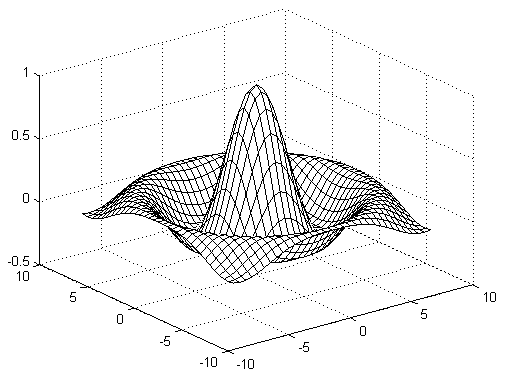
\includegraphics[scale=0.5]{3dmesh}
\centering
\end{figure}

\section{Project Steps}

\begin{enumerate}
\item Update the turtle's logic to compute its movement relative to the three vectors defined above; test this using the existing 2D renderer (simply discard one of the coordinates when rendering)
\item Implement, test, and debug a new 3D renderer using three.js
\item Implement the ability to rotate and move the virtual camera within 3D space
\item Explore applications of the 3D turtle, documenting any interesting ones
\item Explore extensions to the turtle, such as the ability to render with different colors or portray depth
\end{enumerate}

\end{document}
